\documentclass{anstrans}
%%%%%%%%%%%%%%%%%%%%%%%%%%%%%%%%%%%
\title{An Improved ANS Transaction Template}
\author{Baptiste Mouginot,$^{*}$ Kathryn Mummah,$^{*}$ Paul P.H. Wilson$^{*}$}

\institute{
$^{*}$University of Wisconsin-Madison, WI
}

\email{mouginot@wisc.edu \and mummah@wisc.edu \and paul.wilson@wisc.edu}

% Optional disclaimer: remove this command to hide
% \disclaimer{Notice: this manuscript is a work of fiction. Any resemblance to
% actual articles, living or dead, is purely coincidental.}

%%%% packages and definitions (optional)
\usepackage{graphicx} % allows inclusion of graphics
\usepackage{booktabs} % nice rules (thick lines) for tables
\usepackage{microtype} % improves typography for PDF
\usepackage{float}

\newcommand{\SN}{S$_N$}
\renewcommand{\vec}[1]{\bm{#1}} %vector is bold italic
\newcommand{\vd}{\bm{\cdot}} % slightly bold vector dot
\newcommand{\grad}{\vec{\nabla}} % gradient
\newcommand{\ud}{\mathop{}\!\mathrm{d}} % upright derivative symbol

\begin{document}
%%%%%%%%%%%%%%%%%%%%%%%%%%%%%%%%%%%%%%%%%%%%%%%%%%%%%%%%%%%%%%%%%%%%%%%%%%%%%%%%
\section{Introduction}




Some text for introduction etc\ldots
Some text for introduction etc\ldots
Some text for introduction etc\ldots
Some text for introduction etc\ldots
Some text for introduction etc\ldots
Some text for introduction etc\ldots
Some text for introduction etc\ldots
Some text for introduction etc\ldots
Some text for introduction etc\ldots
Some text for introduction etc\ldots
Some text for introduction etc\ldots
Some text for introduction etc\ldots
Some text for introduction etc\ldots
Some text for introduction etc\ldots
Some text for introduction etc\ldots
Some text for introduction etc\ldots
Some text for introduction etc\ldots
Some text for introduction etc\ldots
Some text for introduction etc\ldots
Some text for introduction etc\ldots
Some text for introduction etc\ldots
Some text for introduction etc\ldots
Some text for introduction etc\ldots
Some text for introduction etc\ldots


%%%%%%%%%%%%%%%%%%%%%%%%%%%%%%%%%%%%%%%%%%%%%%%%%%%%%%%%%%%%%%%%%%%%%%%%%%%%%%%%
\section{Theory}



Some text for introduction etc\ldots
Some text for introduction etc\ldots
Some text for introduction etc\ldots
Some text for introduction etc\ldots
Some text for introduction etc\ldots
Some text for introduction etc\ldots
Some text for introduction etc\ldots
Some text for introduction etc\ldots
Some text for introduction etc\ldots
Some text for introduction etc\ldots
Some text for introduction etc\ldots
Some text for introduction etc\ldots
Some text for introduction etc\ldots
Some text for introduction etc\ldots
Some text for introduction etc\ldots
Some text for introduction etc\ldots


\section{Cascade Enrich Construction}
\subsection{Centrifuge properties}
The present work uses the analytical solution by R\"aetz \cite{ref} of the
differential equation for the gas centrifuge as described in \cite{Glaser2008}. Centrifuge parameters, such as average gas temperature, rotation speed, height, feed flow rate, diameter, pressure ratio,
counter-current flow ratio, and efficiency have been chosen to match the cascade design
describe in \cite{glaser2008} and \cite{Walker2017}. These parameters for a P1-type centrifuge are used to estimate the Joint Comprehensive Plan of Action (JCPOA)-compliant IR-1 centrifuge.


\subsection{Cascade Design}

The cascade is built to be ideal, defined by $\alpha =\beta = const$
for all stage of the cascade, where $\alpha$ and $\beta$ respectively represent
the feed to product and the feed to tail enrichment factors.
$\alpha$ can be expressed as a function of the feed rate $F$, the separative performance $\delta U(\theta)$ and $\theta$,
and $\beta$ as a function of $alpha$ and $\theta$:
\begin{subequations} \label{eqs:alphabeta}
    \begin{equation} \label{eq:alpha}
    \alpha = \sqrt{\frac{2\delta U}{F} \frac{1-\theta}{\theta}}+1
\end{equation}
\\
\begin{equation}\label{eq:beta}
    \beta = R
              \dfrac{1 - \dfrac{N - \theta \dfrac{\alpha R}{1+\alpha R}}{1 - \theta}}
                   {\dfrac{N - \theta \dfrac{\alpha R}{1+\alpha R}}{1 - \theta}}
\end{equation}
\end{subequations}

From equation \eqref{eq:alpha} and \eqref{eq:beta} it is possible to determine the cut, or the ratio of product flow to feed flow.
%(all other centrifuge parameters been fixed) allowing the have $\alpha=\beta$
required to build an ideal cascade.

Since $\alpha_{i}$ and $\beta_{i}$ remain constant, only the value of the cut, $\theta_{i}$, changes in each stage of a cascade.

It can be shown that $\theta_{i}$ can be computed from $\alpha$,
$\beta$ values and the feed assay, $N_{i}$ \cite{ref}:
\begin{eqnarray}
    \theta_{i} &=& \dfrac{N_{i} - N''_{i}}{N'_{i}-N''_{i}}\nonumber\\
           &=& \dfrac{N_{i} - \dfrac{1}{1 + \beta/R_{i}}}{ \dfrac{\alpha R_{i}}{1 + \alpha R_{i}} -
           \dfrac{1}{1 + \beta/R_{i}}}
\end{eqnarray}

This algorithm assumes that the corresponding separative power $\delta U$ (not re-computed) can be
achieved with the chosen centrifuge design. Once $\theta_{i}$ determined, it is possible to
compute the product and the tail assay.

The design of the cascade is performed through 2 steps. First one determines the
configuration and number of stages, adding stages following the previously
described procedure, until $N'_{last} > N'_{requested}$ and $N''_{last} <
N''_{requested}$. (Note that $N'_{last}$ corresponds to the product assay of the
last enrichment stage, and $N''_{last}$ to the tail assay of the last stripping
stage). This allows to determine the number of enriching and stripping stages as
well as their enrichment properties ($N_{i}$, $N'_{i}$,
$N''_{i}$,$\theta_{i}$i).
% might be more useful to the reader to say this in words instead of variables, i.e. adding stages until the product assay of the final stage is greater than or equal to than the desired assay, and the tails assay is similarly less than or equal to the desired tails assay

The second step determines how to populate the cascade with the user-defined maximum number of centrifuges. One first solves the linear flow equation to determine the theoretical flow in the
cascade:
\begin{strip}
\begin{equation}
\setcounter{MaxMatrixCols}{20}
\begin{bmatrix}
-1         & 1-\theta_{S+1} & 0              & 0 & ... & 0 & 0            & 0   & 0              & 0 & ... & 0            & 0            & 0 \\
\theta_{S} & -1             & 1-\theta_{S+2} & 0 & ... & 0 & 0            & 0   & 0              & 0 & ... & 0            & 0            & 0 \\
           &                &                &   &     &   &              & ... &                &   &     &              &              &   \\
0          & 0              & 0              & 0 & ... & 0 & \theta_{-1}  & -1  & 1 - \theta_{1} & 0 & ... & 0            & 0            & 0 \\
           &                &                &   &     &   &              & ... &                &   &     &              &              &   \\
0          & 0              & 0              & 0 & ... & 0 & 0            & 0   & 0              & 0 & ... & \theta_{E-2} & -1           & 1-\theta_{E} \\
0          & 0              & 0              & 0 & ... & 0 & 0            & 0   & 0              & 0 & ... & 0            & \theta_{E-1} & -1
\end{bmatrix}
\times
\begin{bmatrix}
     F_{S}   \\
     F_{S+1} \\
     \cdots  \\
     F_{0}   \\
    \cdots   \\
    F_{E-1}  \\
    F_{E}
\end{bmatrix}
=
\begin{bmatrix}
     0   \\
     0 \\
     \cdots  \\
     F   \\
    \cdots   \\
    0  \\
    0
\end{bmatrix}
%\caption{caption needed!}
\label{eq:flow}
\end{equation}
\end{strip}
Once the relative flow of each stage, $F_{i}$, has been determined, the
cascade can be populated with actual machines up the stages
until either the maximum number available of machines or the maximum feed
flow is reached.


\subsection{Response to an non-ideal feed - $\theta_{i} = const$ hypothesis}

Little information is available about the optimum way to tune a cascade that is being fed a feed enrichment that does not match its ideal enrichment.

The tuning method outlined here does not re-optimize $\theta_i$ based on the true flow enrichment. As $\delta
U$ and $\alpha$ do not depend on the stage feed assay $N'$ and the feed to product
ratio $\alpha$ do not change from stage to stage. According to equation
\eqref{eq:beta}, when $\alpha$ and $\theta$ are fixed, if the feed assay,
$N$ changes, then $\beta$ will change accordingly.  This brakes the
ideal status of the cascade, i.e.  $N_{i} \neq N'_{i-1} \neq N''_{i+1}$.

In order to compute the proper product and tails assay at each stages\, the tails and the product from respectively the next and the
previous stage must be blended in order to determine the correct stage feed assay. As this is a
obvious cycling problem, it has been chosen to solve it iteratively: all feed
assay are iteratively updated, blending the proper product and tail, then using
the updated feed assay, the new product and tail assay are recomputed. This
process is repeated until the change in assays is smaller than the
set precision (1e-8 by default).

Other hypotheses will be explored in the future, such as maintaining the ideal
stage of the cascade through tuning the cut values $\theta_{i}$ of each
stage of the cascade, or maintaining $\alpha*\beta = const$ as described in
\cite{walker2017}.

Note that as a consequence of our design method, the cascade product and tail
assay will not necessary match the targeted values, and usually slightly over
enrich and over strip the product and the tail respectively.

\section{The experiment}

As explained previously, the goal of this work is to assess the rate of the highly-enriched uranium (HEU)
production using enrichment cascades designed within the JCPOA agreement
constraints. For this work, two different cases will be investigated and compared
to the reference case.

\subsection{Relevant Cases}
\subsubsection{Reference Case}
The reference case corresponds to the most ideal cascade design--utilizing all the 5060
centrifuges available within JCPOA to produce an enriched product at >$90\%$ of U-235,
stripping the tail product up to 0.28 $\%$ from a feed of natural uranium.
The design cascade in this case, includes 4 stripping stages, and 38 enriching
stages. The Feed/Product/Tail (F/P/T) assay are respectively
0.0071/0.903/0.0028.
%maybe include some cascade shape figures?

\begin{figure}[ht] % replace 't' with 'b' to force it to be on the bottom
  \centering
  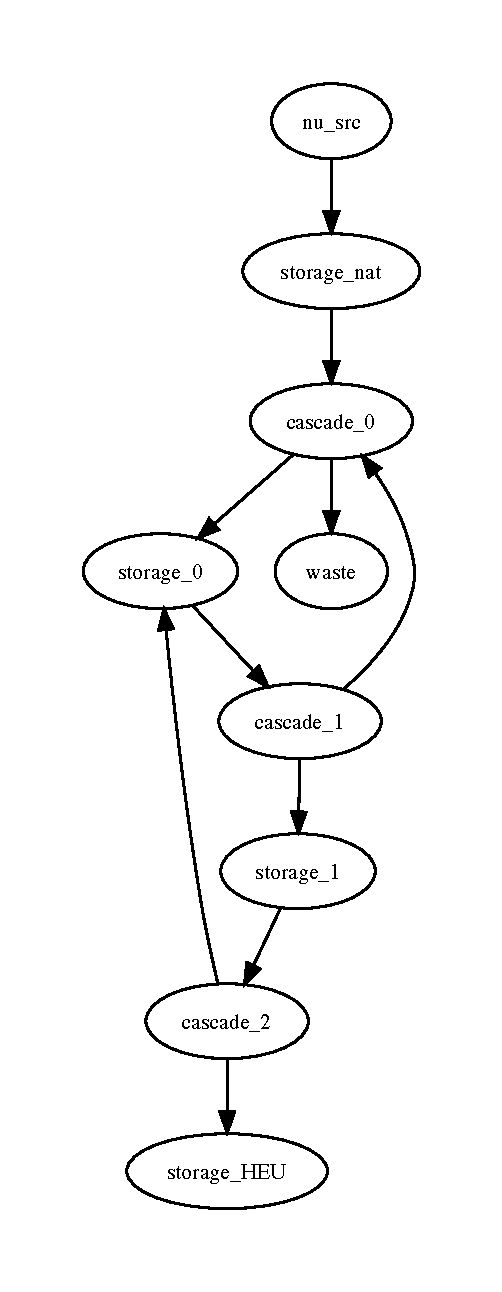
\includegraphics[scale=0.7]{flow_case_2_recy.pdf}
  \caption{Illustraction of the different cascade level materials flow with tail
  recycling.}
  \label{fig:flow}
\end{figure}

\subsubsection{Case 1}
The case 1 is design to allow configure 30 cascades in the scenario (limit of
the JCPOA agreement), all design the same way. The design properties are:\\
- less than 169 centrifuges per cascade,\\
- F/P/T assays: 0.0071/0.035/0.003.\\
The corresponding design is:\\
- 167 centrifuges,\\
- F/P/T assays: 0.0071/0.0412842/0.00290548.\\

\subsubsection{Case 2}
The case 2 is design is also limited to 30 cascades in the scenario (limit of
the JCPOA agreement), but this time each level of cascade are designed to get
feed with the previous level product and to have 4 stripping stages and 10
enriching stages. The configuration of the different level of cascade can be
found in table \ref{tab:cascadelvl}. The different cascades don't have the same
geometry: the number of centrifuges per stage depends on their own design and
varies slightly from a level to another.

\begin{table}[htb]
\centering
\begin{tabular}{cllll}
\toprule

Level   &           & Assay     &       & Machines  \\ 
        & Feed      & Product   & Feed  &           \\
\midrule
1       & 0.0071    & 0.0413    & 0.0029 & 167       \\
2       & 0.0413    & 0.2043    & 0.0173 & 169       \\
3       & 0.2043    & 0.5941    & 0.0971 & 168       \\
4       & 0.5941    & 0.8834    & 0.3915 & 168       \\
5       & 0.8834    & 0.9735    & 0.7746 & 169       \\

\bottomrule
\end{tabular}
  \caption{Summary of the different properties of the different level of cascade.}
  \label{tab:cascadelvl}
\end{table}


\subsection{Level optimisation}
A last round of optimisation if then ran in order to limit the number of cascade
level to the amount of level required produce HEU, and then to populate the
different level with a total of 30 cascades in order to maximize the HEU
production rate.

\section{Results}
\subsection{Enrichment}
\subsubsection{Without tail recycling}
Despite the reconfiguration of each level occuring in the second case, the case
1 is way more effective to produce HEU than case 1.
Indeed as observed on Figure \ref{} and \ref{}, the first case is able to
produce a an uranium product enrich at $98\%$ while the second case is only able
to reach an enrichment of $88.3\%$.
This is the consequence of the usage of un-touched cascade in the case 1:
because the cut value at each stage is unchanged it artificially produces over
enricht tails when feeded with higher enriched materials compared to a cascade
feed with the same feed assay but with a cascade designed for it.
The effective cut values for each cascade can be computed as :
\begin{equation}\label{eq:theta_eff}
    \theta = \dfrac{N - N''}{N'-N''}
\end{equation}

\begin{table}[htb]
\centering
\begin{tabular}{cll}
\toprule

Level   &  $\theta_{eff}^{C1}$   & $\theta_{eff}^{C2}$ \\ 
\midrule
1       & 0.109375               & 0.109375     \\
2       & 0.109375               & 0.128342     \\
3       & 0.109375               & 0.215694     \\
4       & 0.109375               & 0.411872     \\
5       & 0.109375               & 0.547009     \\

\bottomrule
\end{tabular}
  \caption{Cascade effective $\theta$ as a function of the cascade level and the
  case considered.}
  \label{tab:cascade_theta}
\end{table}
As illustrated on Table \ref{tab:cascade_theta} the effecive cut of the the
different level increase up to $0.54$ for the fifth stage on case 2. The high
effecive cut value increase the product production rate but decrease the
enrichment ratio.

\subsubsection{tails recycling}
\subsubsection{Case 1}
As shows on Figure \ref{ }, without tails recycling, the number of cascade level
required to enrich the uranium up to $90\%$ are respectively 5 for the
first case considered. Recycling the tails, allow to reduce the number of
enrichment levels required to enrich natural uranium up to a high enrich level
to 3.

This bump in enrichment can easily be explained, as the cascade does not have the
same number of stages, there is less stripping enrichment work, than enriching
work. That is to say that even work in an ideal case (where the stripping work of a
stage is the exact inverse of the enrich work), with an cascade with less
stripping stage than enriching stage will produce tail with a higher enrichment
than the feed of the previous level of


%%%%%%%%%%%%%%%%%%%%%%%%%%%%%%%%%%%%%%%%%%%%%%%%%%%%%%%%%%%%%%%%%%%%%%%%%%%%%%%%
\section{Results and Analysis}

%%%%%%%%%%%%%%%%%%%%%%%%%%%%%%%%%%%%%%%%%%%%%%%%%%%%%%%%%%%%%%%%%%%%%%%%%%%%%%%%
\subsection{Subsection Goes Here}
\begin{equation} \label{eq:marshak}
  4 J^- = \phi + 2 D \vec{n} \vd \grad \phi \,.
\end{equation}
If we so choose, we can effortlessly reference the equation later.

\begin{figure}[ht] % replace 't' with 'b' to force it to be on the bottom
  \centering
  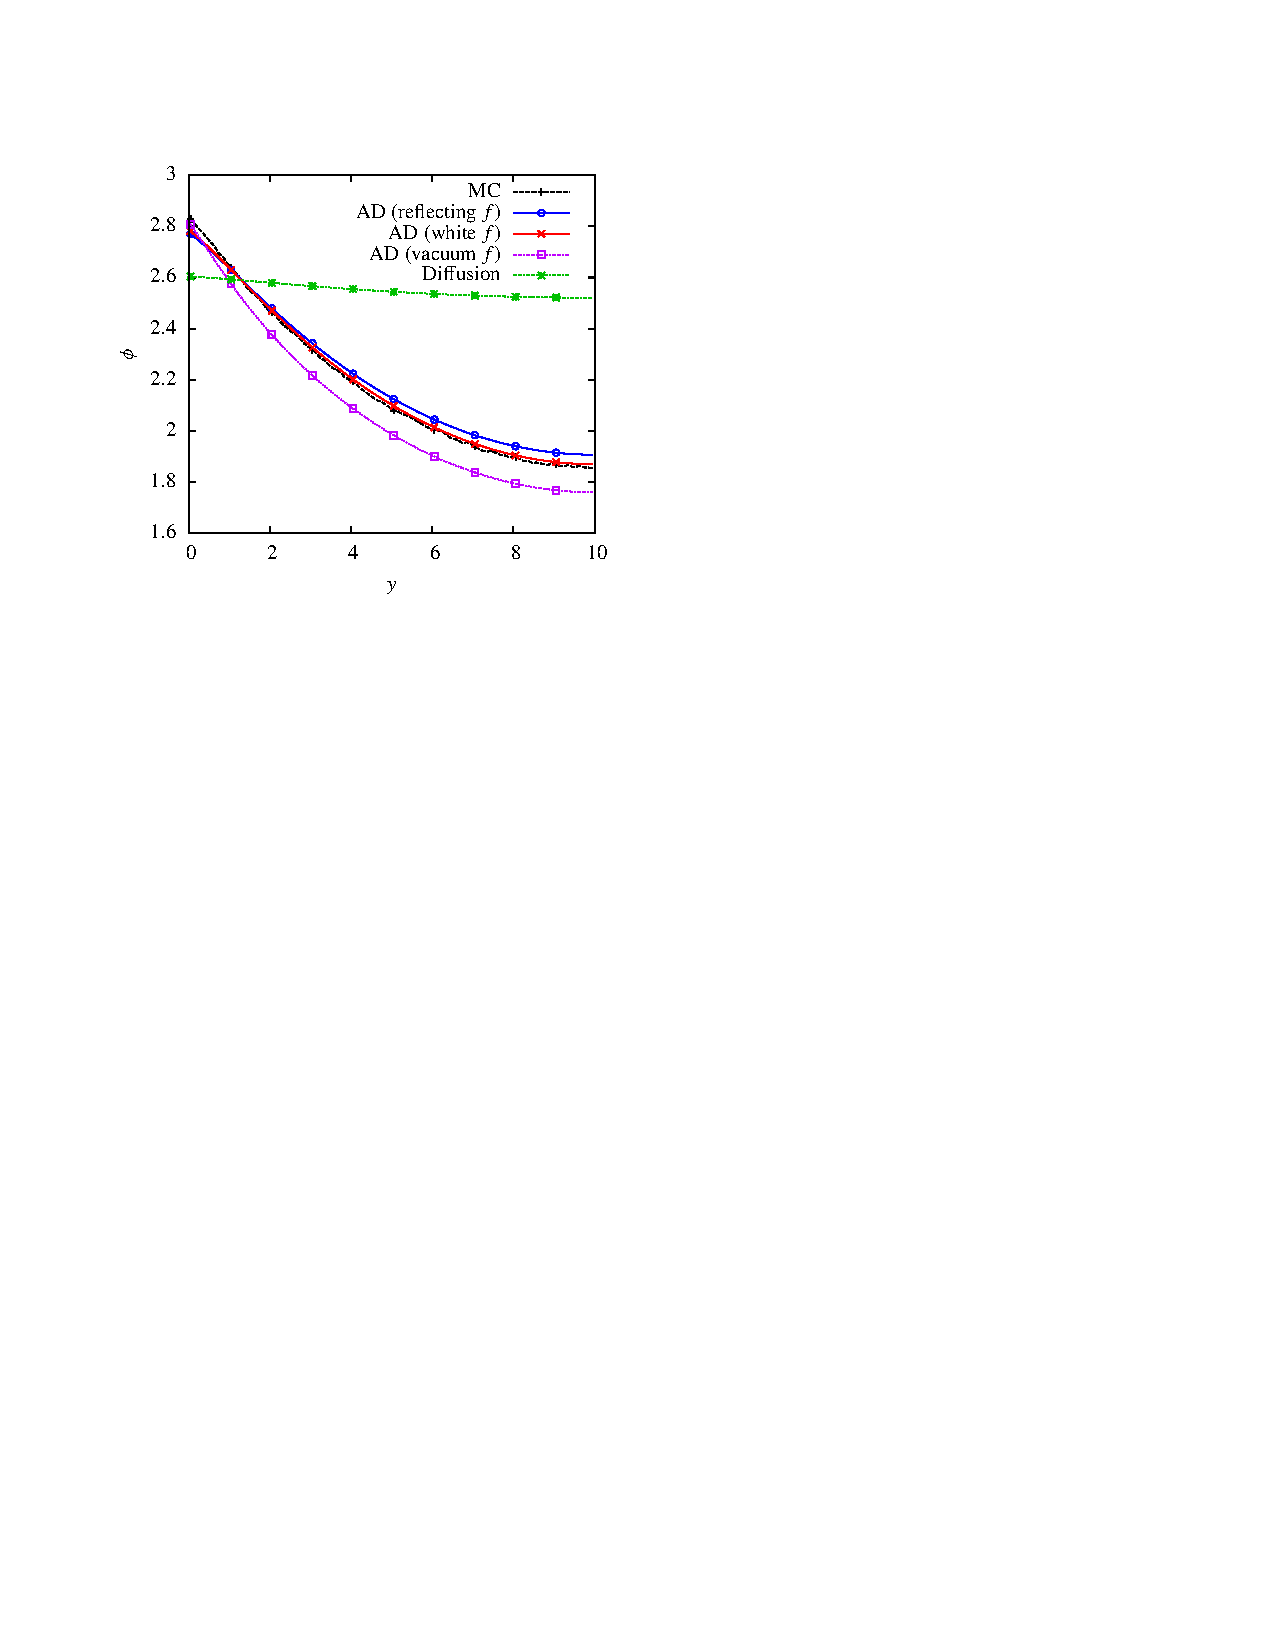
\includegraphics{example_figure}
  \caption{Captions are flush with the left.}
  \label{fig:voltage}
\end{figure}

Later on, we can include a table, even one that spans two columns such as
Table~\ref{tab:widetable}.
%%%%%%%%%%%%%%%%%%%%%%%%%%%%%%%%%%%%%%%%
%%%%%%%%%%%%%%%%%%%%%%%%%%%%%%%%%%%%%%%%
Notice how the table reference uses a Roman numeral
for its numbering scheme, whereas the figure reference uses an Arabic numeral.
For one-column tables, use the \verb|table| environment; two-column tables use
\verb|table*|. The same applies to figures.

%%%%%%%%%%%%%%%%%%%%%%%%%%%%%%%%%%%%%%%%%%%%%%%%%%%%%%%%%%%%%%%%%%%%%%%%%%%%%%%%
\subsection{Another Subsection}
Excessive sectioning in a three-page document is discouraged, but here are more
subsections to demonstrate compliance with the ANS formatting guidelines.

\subsubsection{Third-level Heading}
This subsubsection shows compliance with the ANS-specified standard. This level
of heading should be used rarely.

\subsubsection{Another Such Heading}
And, if you really think you need a third-level heading, you should make sure
that your subsection needs at least two of them.

%%%%%%%%%%%%%%%%%%%%%%%%%%%%%%%%%%%%%%%%%%%%%%%%%%%%%%%%%%%%%%%%%%%%%%%%%%%%%%%%
\section{Conclusions}

The included ANS style file and this clear example file are a panacea for
the hours of headache that invariably results from formatting a document in
Microsoft Word.

%%%%%%%%%%%%%%%%%%%%%%%%%%%%%%%%%%%%%%%%%%%%%%%%%%%%%%%%%%%%%%%%%%%%%%%%%%%%%%%%
\appendix
\section{Appendix}

Numbering in the appendix is different:
\begin{equation} \label{eq:appendix}
  2 + 2 = 5\,.
\end{equation}
and another equation:
\begin{equation} \label{eq:appendix2}
  a + b = c\,.
\end{equation}

%%%%%%%%%%%%%%%%%%%%%%%%%%%%%%%%%%%%%%%%%%%%%%%%%%%%%%%%%%%%%%%%%%%%%%%%%%%%%%%%
\section{Nomenclature}

\begin{table}[H]
    \centering
    \begin{tabular}{l|l}
%         &  \\
        $N$ & Feed assay \\
        $N'$ & Product assay \\
        $N''$ & Tails assay \\
        $\alpha$ & Feed to product enrichment factor \\
        $\beta$ & Feed to tail enrichment factor \\
        $\theta$ & Cut
    \end{tabular}
%    \caption{Caption}
    \label{tab:my_label}
\end{table}

%%%%%%%%%%%%%%%%%%%%%%%%%%%%%%%%%%%%%%%%%%%%%%%%%%%%%%%%%%%%%%%%%%%%%%%%%%%%%%%%
\section{Acknowledgments}
This material is based upon work supported a Department of Energy Nuclear
Energy University Programs Graduate Fellowship.

%%%%%%%%%%%%%%%%%%%%%%%%%%%%%%%%%%%%%%%%%%%%%%%%%%%%%%%%%%%%%%%%%%%%%%%%%%%%%%%%
\bibliographystyle{ans}
\bibliography{bibliography}
\end{document}
